\documentclass[border=10pt]{standalone}
\usepackage[svgnames]{xcolor}
\usepackage{amsmath}
\usepackage{pgfplots}
\pgfplotsset{compat=newest}
\usepackage[sfdefault]{FiraSans}
\usepackage{FiraMono}
\renewcommand*\familydefault{\sfdefault}
\begin{document}
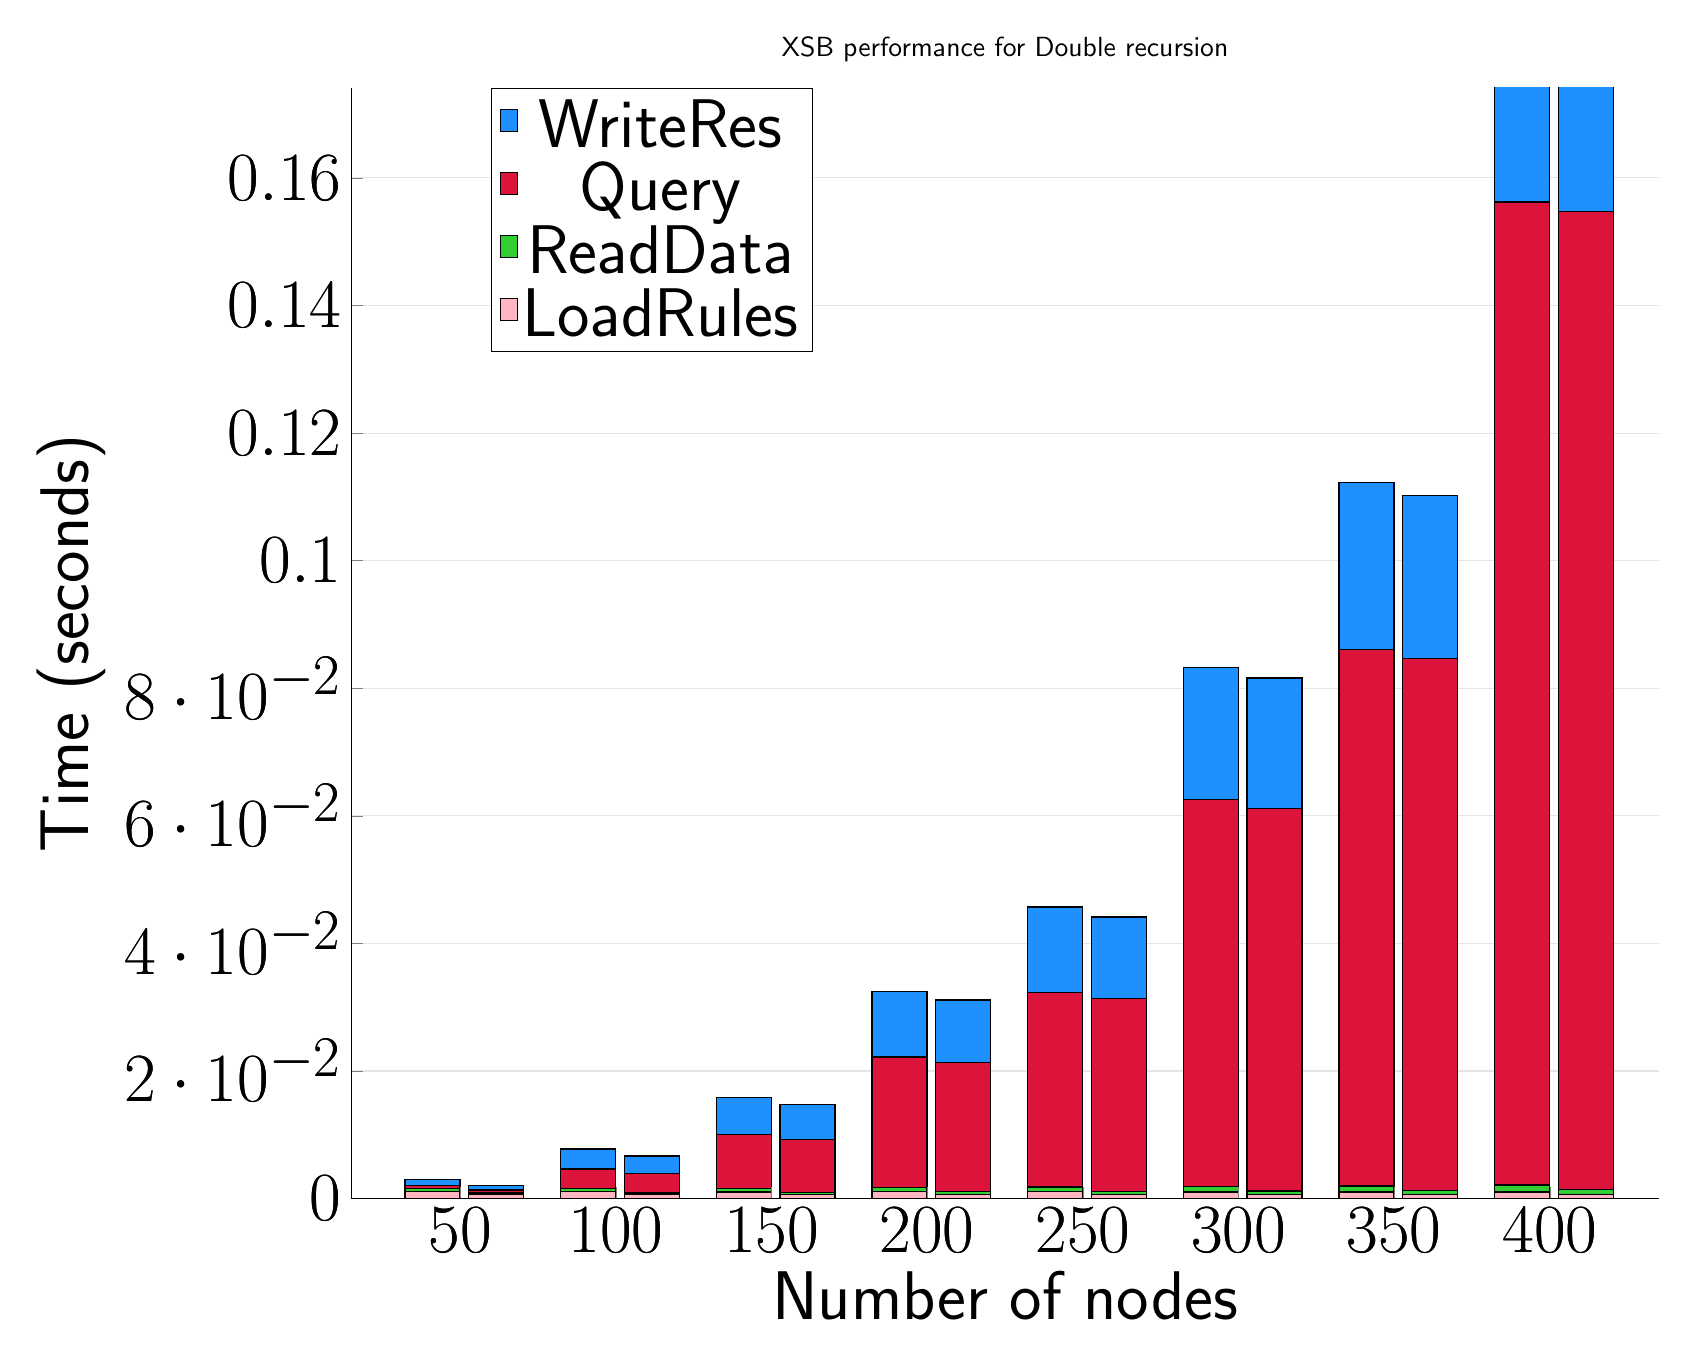
\begin{tikzpicture}
\begin{axis}[
   ybar stacked,
   title={XSB performance for Double recursion},
   bar shift=-10pt,
   width=1.5\textwidth,
   bar width=0.7cm,
   ymajorgrids, tick align=inside,
   major grid style={draw=gray!20},
   xtick=data,
   ymin=0, ymax=0.1741104793548585,
   axis x line*=bottom,
   axis y line*=left,
   enlarge x limits=0.1,
   legend style={
       at={(0.23, 1)},
       anchor=north,
       legend columns=1,
       font=\Huge,
   },
   ylabel={Time (seconds)},
   xlabel={Number of nodes},
   label style={font=\Huge},
   tick label style={font=\Huge},
]
\addlegendimage{fill=DodgerBlue, draw=black, line width=0.2pt}
\addlegendentry{WriteRes}
\addlegendimage{fill=Crimson, draw=black, line width=0.2pt}
\addlegendentry{Query}
\addlegendimage{fill=LimeGreen, draw=black, line width=0.2pt}
\addlegendentry{ReadData}
\addlegendimage{fill=LightPink, draw=black, line width=0.2pt}
\addlegendentry{LoadRules}
\addplot +[fill=LightPink, draw=black, line width=0.5pt] coordinates {
    (50, 0.0011386632919311531)
    (100, 0.0010604143142700201)
    (150, 0.001047396659851075)
    (200, 0.0010972976684570322)
    (250, 0.0010708808898925771)
    (300, 0.001049733161926271)
    (350, 0.0010429859161376947)
    (400, 0.0010591030120849598)
};
\addplot +[fill=LimeGreen, draw=black, line width=0.5pt] coordinates {
    (50, 0.00042793750762939455)
    (100, 0.0004880189895629883)
    (150, 0.0005707025527954101)
    (200, 0.0006756782531738279)
    (250, 0.0007190227508544921)
    (300, 0.0008332014083862304)
    (350, 0.0009128093719482418)
    (400, 0.0010400056838989267)
};
\addplot +[fill=Crimson, draw=black, line width=0.5pt] coordinates {
    (50, 0.00047240257263183585)
    (100, 0.003065180778503416)
    (150, 0.008391642570495605)
    (200, 0.020405745506286634)
    (250, 0.03049008846282959)
    (300, 0.06069538593292236)
    (350, 0.08414080142974853)
    (400, 0.1541104793548585)
};
\addplot +[fill=DodgerBlue, draw=black, line width=0.5pt] coordinates {
    (50, 0.0009920120239257822)
    (100, 0.0031403303146362313)
    (150, 0.0058816671371459735)
    (200, 0.01027448177337645)
    (250, 0.01344199180603028)
    (300, 0.02070729732513427)
    (350, 0.02615497112274176)
    (400, 0.04116942882537831)
};
\end{axis}
\begin{axis}[
   ybar stacked,
   bar shift=13pt,
   width=1.5\textwidth,
   bar width=0.7cm,
   ymajorgrids, tick align=inside,
   major grid style={draw=none},
   xtick=data,
   ymin=0, ymax=0.1741104793548585,
   axis x line*=none,
   axis y line*=none,
   enlarge x limits=0.1,
   label style={font=\Huge},
   tick label style={font=\Huge},
]
\addplot +[fill=LightPink, draw=black, line width=0.5pt] coordinates {
    (50, 0.0006374999999999995)
    (100, 0.0006148000000000002)
    (150, 0.0006026000000000001)
    (200, 0.0006316000000000006)
    (250, 0.0006133000000000004)
    (300, 0.0006089000000000007)
    (350, 0.0006050000000000002)
    (400, 0.0006096999999999995)
};
\addplot +[fill=LimeGreen, draw=black, line width=0.5pt] coordinates {
    (50, 0.0002209000000000006)
    (100, 0.0002868000000000001)
    (150, 0.00035640000000000004)
    (200, 0.0004567999999999994)
    (250, 0.0004945999999999998)
    (300, 0.0006055999999999995)
    (350, 0.0006771999999999999)
    (400, 0.0007857999999999997)
};
\addplot +[fill=Crimson, draw=black, line width=0.5pt] coordinates {
    (50, 0.0004575999999999997)
    (100, 0.0030108)
    (150, 0.0083033)
    (200, 0.0202289)
    (250, 0.030231100000000004)
    (300, 0.059918799999999994)
    (350, 0.08338500000000001)
    (400, 0.15335130000000002)
};
\addplot +[fill=DodgerBlue, draw=black, line width=0.5pt] coordinates {
    (50, 0.0007342000000000003)
    (100, 0.0027848)
    (150, 0.0055319)
    (200, 0.009837799999999999)
    (250, 0.0127906)
    (300, 0.0204645)
    (350, 0.025584600000000002)
    (400, 0.040078499999999996)
};
\end{axis}
\end{tikzpicture}

\end{document}
